\documentclass[twoside]{book}

% Packages required by doxygen
\usepackage{calc}
\usepackage{doxygen}
\usepackage{graphicx}
\usepackage[utf8]{inputenc}
\usepackage{makeidx}
\usepackage{multicol}
\usepackage{multirow}
\usepackage{textcomp}
\usepackage[table]{xcolor}

% Font selection
\usepackage[T1]{fontenc}
\usepackage{mathptmx}
\usepackage[scaled=.90]{helvet}
\usepackage{courier}
\usepackage{amssymb}
\usepackage{sectsty}
\renewcommand{\familydefault}{\sfdefault}
\allsectionsfont{%
  \fontseries{bc}\selectfont%
  \color{darkgray}%
}
\renewcommand{\DoxyLabelFont}{%
  \fontseries{bc}\selectfont%
  \color{darkgray}%
}

% Page & text layout
\usepackage{geometry}
\geometry{%
  a4paper,%
  top=2.5cm,%
  bottom=2.5cm,%
  left=2.5cm,%
  right=2.5cm%
}
\tolerance=750
\hfuzz=15pt
\hbadness=750
\setlength{\emergencystretch}{15pt}
\setlength{\parindent}{0cm}
\setlength{\parskip}{0.2cm}
\makeatletter
\renewcommand{\paragraph}{%
  \@startsection{paragraph}{4}{0ex}{-1.0ex}{1.0ex}{%
    \normalfont\normalsize\bfseries\SS@parafont%
  }%
}
\renewcommand{\subparagraph}{%
  \@startsection{subparagraph}{5}{0ex}{-1.0ex}{1.0ex}{%
    \normalfont\normalsize\bfseries\SS@subparafont%
  }%
}
\makeatother

% Headers & footers
\usepackage{fancyhdr}
\pagestyle{fancyplain}
\fancyhead[LE]{\fancyplain{}{\bfseries\thepage}}
\fancyhead[CE]{\fancyplain{}{}}
\fancyhead[RE]{\fancyplain{}{\bfseries\leftmark}}
\fancyhead[LO]{\fancyplain{}{\bfseries\rightmark}}
\fancyhead[CO]{\fancyplain{}{}}
\fancyhead[RO]{\fancyplain{}{\bfseries\thepage}}
\fancyfoot[LE]{\fancyplain{}{}}
\fancyfoot[CE]{\fancyplain{}{}}
\fancyfoot[RE]{\fancyplain{}{\bfseries\scriptsize Generated on Sat Sep 3 2016 19\-:38\-:37 for A\-I\-D\-A analysis software by Doxygen }}
\fancyfoot[LO]{\fancyplain{}{\bfseries\scriptsize Generated on Sat Sep 3 2016 19\-:38\-:37 for A\-I\-D\-A analysis software by Doxygen }}
\fancyfoot[CO]{\fancyplain{}{}}
\fancyfoot[RO]{\fancyplain{}{}}
\renewcommand{\footrulewidth}{0.4pt}
\renewcommand{\chaptermark}[1]{%
  \markboth{#1}{}%
}
\renewcommand{\sectionmark}[1]{%
  \markright{\thesection\ #1}%
}

% Indices & bibliography
\usepackage{natbib}
\usepackage[titles]{tocloft}
\setcounter{tocdepth}{3}
\setcounter{secnumdepth}{5}
\makeindex

% Hyperlinks (required, but should be loaded last)
\usepackage{ifpdf}
\ifpdf
  \usepackage[pdftex,pagebackref=true]{hyperref}
\else
  \usepackage[ps2pdf,pagebackref=true]{hyperref}
\fi
\hypersetup{%
  colorlinks=true,%
  linkcolor=blue,%
  citecolor=blue,%
  unicode%
}

% Custom commands
\newcommand{\clearemptydoublepage}{%
  \newpage{\pagestyle{empty}\cleardoublepage}%
}


%===== C O N T E N T S =====

\begin{document}

% Titlepage & ToC
\hypersetup{pageanchor=false}
\pagenumbering{roman}
\begin{titlepage}
\vspace*{7cm}
\begin{center}%
{\Large A\-I\-D\-A analysis software \\[1ex]\large 0 }\\
\vspace*{1cm}
{\large Generated by Doxygen 1.8.5}\\
\vspace*{0.5cm}
{\small Sat Sep 3 2016 19:38:37}\\
\end{center}
\end{titlepage}
\clearemptydoublepage
\tableofcontents
\clearemptydoublepage
\pagenumbering{arabic}
\hypersetup{pageanchor=true}

%--- Begin generated contents ---
\chapter{Hierarchical Index}
\section{Class Hierarchy}
This inheritance list is sorted roughly, but not completely, alphabetically\-:\begin{DoxyCompactList}
\item \contentsline{section}{Analysis}{\pageref{classAnalysis}}{}
\item \contentsline{section}{Calibrator}{\pageref{classCalibrator}}{}
\item \contentsline{section}{Data\-Source}{\pageref{classDataSource}}{}
\item T\-Signal\-Handler\begin{DoxyCompactList}
\item \contentsline{section}{My\-Signal\-Handler}{\pageref{classMySignalHandler}}{}
\end{DoxyCompactList}
\item \contentsline{section}{Unpacker}{\pageref{classUnpacker}}{}
\end{DoxyCompactList}

\chapter{Class Index}
\section{Class List}
Here are the classes, structs, unions and interfaces with brief descriptions\-:\begin{DoxyCompactList}
\item\contentsline{section}{\hyperlink{classAnalysis}{Analysis} \\*A brief description of the class }{\pageref{classAnalysis}}{}
\item\contentsline{section}{\hyperlink{classCalibrator}{Calibrator} }{\pageref{classCalibrator}}{}
\item\contentsline{section}{\hyperlink{classDataSource}{Data\-Source} }{\pageref{classDataSource}}{}
\item\contentsline{section}{\hyperlink{classMySignalHandler}{My\-Signal\-Handler} }{\pageref{classMySignalHandler}}{}
\item\contentsline{section}{\hyperlink{classUnpacker}{Unpacker} }{\pageref{classUnpacker}}{}
\end{DoxyCompactList}

\chapter{File Index}
\section{File List}
Here is a list of all documented files with brief descriptions\-:\begin{DoxyCompactList}
\item\contentsline{section}{include/\hyperlink{Analysis_8h}{Analysis.\-h} }{\pageref{Analysis_8h}}{}
\item\contentsline{section}{include/{\bfseries c\-\_\-functions.\-h} }{\pageref{c__functions_8h}}{}
\item\contentsline{section}{include/{\bfseries Calibrator.\-h} }{\pageref{Calibrator_8h}}{}
\item\contentsline{section}{include/{\bfseries Common.\-h} }{\pageref{Common_8h}}{}
\item\contentsline{section}{include/{\bfseries Data\-Source.\-h} }{\pageref{DataSource_8h}}{}
\item\contentsline{section}{include/{\bfseries kbhit.\-h} }{\pageref{kbhit_8h}}{}
\item\contentsline{section}{include/{\bfseries My\-Signal\-Handler.\-h} }{\pageref{MySignalHandler_8h}}{}
\item\contentsline{section}{include/{\bfseries Unpacker.\-h} }{\pageref{Unpacker_8h}}{}
\item\contentsline{section}{src/\hyperlink{Analysis_8cpp}{Analysis.\-cpp} }{\pageref{Analysis_8cpp}}{}
\end{DoxyCompactList}

\chapter{Class Documentation}
\hypertarget{classAnalysis}{\section{Analysis Class Reference}
\label{classAnalysis}\index{Analysis@{Analysis}}
}


A brief description of the class.  




{\ttfamily \#include $<$Analysis.\-h$>$}

\subsection*{Public Member Functions}
\begin{DoxyCompactItemize}
\item 
\hypertarget{classAnalysis_a88fe5552815cc257f3acd801e46c7046}{void {\bfseries Init\-Analysis} (int opt)}\label{classAnalysis_a88fe5552815cc257f3acd801e46c7046}

\item 
\hypertarget{classAnalysis_afae21198450b4b553a1a7750b4644659}{void {\bfseries Process} (\hyperlink{classDataSource}{Data\-Source} \&my\-\_\-source, \hyperlink{classCalibrator}{Calibrator} \&my\-\_\-cal\-\_\-data)}\label{classAnalysis_afae21198450b4b553a1a7750b4644659}

\item 
\hypertarget{classAnalysis_a8f737475bbb30bc543f3b5c920072876}{void {\bfseries Close} ()}\label{classAnalysis_a8f737475bbb30bc543f3b5c920072876}

\item 
\hypertarget{classAnalysis_af920e254681982b5ff2a8062a66b10fb}{bool {\bfseries Build\-Event} (\hyperlink{classCalibrator}{Calibrator} \&my\-\_\-cal\-\_\-data)}\label{classAnalysis_af920e254681982b5ff2a8062a66b10fb}

\item 
\hypertarget{classAnalysis_a5bad79058d6d56097d7f6be84372da87}{void {\bfseries Close\-Event} ()}\label{classAnalysis_a5bad79058d6d56097d7f6be84372da87}

\item 
\hypertarget{classAnalysis_a6756b25d7564dfe09920293295d542e5}{void {\bfseries Init\-Event} (\hyperlink{classCalibrator}{Calibrator} \&my\-\_\-cal\-\_\-data)}\label{classAnalysis_a6756b25d7564dfe09920293295d542e5}

\item 
\hypertarget{classAnalysis_a770471b4eaadf5e8b68f1d9231d2a51f}{void {\bfseries Fill\-Histograms\-Singles} (\hyperlink{classCalibrator}{Calibrator} \&my\-\_\-cal\-\_\-data)}\label{classAnalysis_a770471b4eaadf5e8b68f1d9231d2a51f}

\item 
\hypertarget{classAnalysis_aac936a81400f18975af55043a8462fea}{void {\bfseries Fill\-Histograms\-Event} ()}\label{classAnalysis_aac936a81400f18975af55043a8462fea}

\item 
\hypertarget{classAnalysis_a5c82e57f8a238d847b603d6ee096f16b}{void {\bfseries Update\-Histograms} ()}\label{classAnalysis_a5c82e57f8a238d847b603d6ee096f16b}

\item 
\hypertarget{classAnalysis_a5cb6bccbd5c0ddaaf9a3c6ed216352f6}{void {\bfseries Reset\-Histograms} ()}\label{classAnalysis_a5cb6bccbd5c0ddaaf9a3c6ed216352f6}

\item 
\hypertarget{classAnalysis_ac63c498af33d55526e4faf89ff4aed72}{void {\bfseries Reset\-Event} ()}\label{classAnalysis_ac63c498af33d55526e4faf89ff4aed72}

\item 
\hypertarget{classAnalysis_acd5f9382c18b82835431ba127ff79a6c}{void {\bfseries Write\-Histograms} ()}\label{classAnalysis_acd5f9382c18b82835431ba127ff79a6c}

\item 
\hypertarget{classAnalysis_a5bde2aa071c458976fd4d90e8f577fb7}{void {\bfseries Write\-Out\-Buffer} (\hyperlink{classDataSource}{Data\-Source} \&my\-\_\-source)}\label{classAnalysis_a5bde2aa071c458976fd4d90e8f577fb7}

\item 
\hypertarget{classAnalysis_a2b12b00bda7f6a53ac0d7eb8b6a9f98b}{bool {\bfseries Is\-Ch\-Enabled} (\hyperlink{classCalibrator}{Calibrator} \&my\-\_\-cal\-\_\-data)}\label{classAnalysis_a2b12b00bda7f6a53ac0d7eb8b6a9f98b}

\item 
\hypertarget{classAnalysis_a40784904bec827cc7a6a34b01d7d148c}{bool {\bfseries Set\-Event\-Time\-Window} (double value)}\label{classAnalysis_a40784904bec827cc7a6a34b01d7d148c}

\item 
\hypertarget{classAnalysis_aee81123c9bd56f06468e9b0da9230803}{void {\bfseries Print\-Event} ()}\label{classAnalysis_aee81123c9bd56f06468e9b0da9230803}

\item 
\hypertarget{classAnalysis_aace40580ef23453e3bfb1075554e076e}{void {\bfseries Set\-B\-Debug} (bool flag)}\label{classAnalysis_aace40580ef23453e3bfb1075554e076e}

\item 
\hypertarget{classAnalysis_af13631304f9dbfe58969c179da01ee9e}{void {\bfseries Set\-B\-Histograms} (bool flag)}\label{classAnalysis_af13631304f9dbfe58969c179da01ee9e}

\item 
\hypertarget{classAnalysis_a63975fb6e4fb62fa5b0d07dc012e6499}{void {\bfseries Set\-B\-Push\-Data} (bool flag)}\label{classAnalysis_a63975fb6e4fb62fa5b0d07dc012e6499}

\item 
\hypertarget{classAnalysis_a6d1d4d2b7149f4088e58b72c8dfbc13f}{void {\bfseries Set\-B\-Fill\-Tree} (bool flag)}\label{classAnalysis_a6d1d4d2b7149f4088e58b72c8dfbc13f}

\item 
\hypertarget{classAnalysis_a0138f49287e2d44baa42ba9f9b9aca28}{void {\bfseries Set\-B\-Root\-Tree} (bool flag)}\label{classAnalysis_a0138f49287e2d44baa42ba9f9b9aca28}

\item 
\hypertarget{classAnalysis_a436525d257c88b218ea51485d101b267}{double {\bfseries Get\-Event\-Time\-Window} ()}\label{classAnalysis_a436525d257c88b218ea51485d101b267}

\item 
\hypertarget{classAnalysis_a0da01bf0e0aa34f4ae76bd94db0d09c1}{bool {\bfseries Get\-B\-Debug} ()}\label{classAnalysis_a0da01bf0e0aa34f4ae76bd94db0d09c1}

\item 
\hypertarget{classAnalysis_afbb0dbe1487bfcdad2d9c38c149f27e0}{bool {\bfseries Get\-B\-Histograms} ()}\label{classAnalysis_afbb0dbe1487bfcdad2d9c38c149f27e0}

\item 
\hypertarget{classAnalysis_a866f4560f2145d0e8059db476d3df186}{bool {\bfseries Get\-B\-Push\-Data} ()}\label{classAnalysis_a866f4560f2145d0e8059db476d3df186}

\item 
\hypertarget{classAnalysis_af764dca2c23b49900454d617196fe498}{bool {\bfseries Get\-B\-Fill\-Tree} ()}\label{classAnalysis_af764dca2c23b49900454d617196fe498}

\item 
\hypertarget{classAnalysis_abf7fe1c81f379e071616d45b4b6a3d99}{bool {\bfseries Get\-B\-Root\-Tree} ()}\label{classAnalysis_abf7fe1c81f379e071616d45b4b6a3d99}

\item 
\hypertarget{classAnalysis_aa2cf8de2ad8ed44580e741e482a886af}{int {\bfseries Get\-Multiplicity} ()}\label{classAnalysis_aa2cf8de2ad8ed44580e741e482a886af}

\end{DoxyCompactItemize}
\subsection*{Public Attributes}
\begin{DoxyCompactItemize}
\item 
\hypertarget{classAnalysis_a4563c7dc9e8dc450dd5652947123a6ee}{T\-H2\-I $\ast$ \hyperlink{classAnalysis_a4563c7dc9e8dc450dd5652947123a6ee}{h\-A\-D\-Clow\-Ch} \mbox{[}common\-::\-N\-\_\-\-F\-E\-E64\mbox{]}}\label{classAnalysis_a4563c7dc9e8dc450dd5652947123a6ee}

\begin{DoxyCompactList}\small\item\em N\-\_\-\-F\-E\-E64 D array of T\-H2\-I$\ast$ graphing A\-D\-C spectrum in 2\-D for low energy range. \end{DoxyCompactList}\item 
\hypertarget{classAnalysis_ae0292c6dffdfcc8ab15c296b1553829e}{T\-H2\-I $\ast$ \hyperlink{classAnalysis_ae0292c6dffdfcc8ab15c296b1553829e}{h\-A\-D\-Chigh\-Ch} \mbox{[}common\-::\-N\-\_\-\-F\-E\-E64\mbox{]}}\label{classAnalysis_ae0292c6dffdfcc8ab15c296b1553829e}

\begin{DoxyCompactList}\small\item\em N\-\_\-\-F\-E\-E64 D array of T\-H2\-I$\ast$ graphing A\-D\-C spectrum in 2\-D for high energy range. \end{DoxyCompactList}\item 
\hypertarget{classAnalysis_afcc03dd184a24fe5b33d053ba54a0438}{T\-H2\-I $\ast$ \hyperlink{classAnalysis_afcc03dd184a24fe5b33d053ba54a0438}{h\-A\-D\-Cdisc\-Ch} \mbox{[}common\-::\-N\-\_\-\-F\-E\-E64\mbox{]}}\label{classAnalysis_afcc03dd184a24fe5b33d053ba54a0438}

\begin{DoxyCompactList}\small\item\em N\-\_\-\-F\-E\-E64 D array of T\-H2\-I$\ast$ graphing A\-D\-C spectrum in 2\-D for fast discriminator. \end{DoxyCompactList}\item 
\hypertarget{classAnalysis_aec6281344bd8ee77b392f168defb858e}{T\-H1\-I $\ast$ \hyperlink{classAnalysis_aec6281344bd8ee77b392f168defb858e}{h\-Ch\-\_\-\-A\-D\-Clow} \mbox{[}common\-::\-N\-\_\-\-F\-E\-E64\mbox{]}}\label{classAnalysis_aec6281344bd8ee77b392f168defb858e}

\begin{DoxyCompactList}\small\item\em N\-\_\-\-F\-E\-E64 D array of T\-H1\-I$\ast$ graphing A\-D\-C spectrum in 1\-D for low energy range. \end{DoxyCompactList}\item 
\hypertarget{classAnalysis_a10ff082c45fa557c4531e9586d45e31c}{T\-H1\-I $\ast$ \hyperlink{classAnalysis_a10ff082c45fa557c4531e9586d45e31c}{h\-Ch\-\_\-\-A\-D\-Chigh} \mbox{[}common\-::\-N\-\_\-\-F\-E\-E64\mbox{]}}\label{classAnalysis_a10ff082c45fa557c4531e9586d45e31c}

\begin{DoxyCompactList}\small\item\em N\-\_\-\-F\-E\-E64 D array of T\-H1\-I$\ast$ graphing A\-D\-C spectrum in 1\-D for high energy range. \end{DoxyCompactList}\item 
\hypertarget{classAnalysis_a41545602157ccbdfafa902ab8cc675e0}{T\-H1\-I $\ast$ \hyperlink{classAnalysis_a41545602157ccbdfafa902ab8cc675e0}{h\-Ch\-\_\-\-A\-D\-Cdisc} \mbox{[}common\-::\-N\-\_\-\-F\-E\-E64\mbox{]}}\label{classAnalysis_a41545602157ccbdfafa902ab8cc675e0}

\begin{DoxyCompactList}\small\item\em N\-\_\-\-F\-E\-E64 D array of T\-H1\-I$\ast$ graphing A\-D\-C spectrum in 1\-D for fast discriminator. \end{DoxyCompactList}\item 
\hypertarget{classAnalysis_af017884cee08db1ec1358fe4d3424aca}{T\-H1\-I $\ast$ \hyperlink{classAnalysis_af017884cee08db1ec1358fe4d3424aca}{h\-A\-D\-Clow\-\_\-all} \mbox{[}common\-::\-N\-\_\-\-D\-S\-S\-D\mbox{]}}\label{classAnalysis_af017884cee08db1ec1358fe4d3424aca}

\begin{DoxyCompactList}\small\item\em N\-\_\-\-D\-S\-S\-D D array of T\-H1\-I$\ast$ graphing A\-D\-C combined A\-D\-C spectrum of calibrated strips for whole D\-S\-S\-D. \end{DoxyCompactList}\item 
\hypertarget{classAnalysis_ae38834865c6f470c5e456b05481ad142}{T\-H1\-I $\ast$ \hyperlink{classAnalysis_ae38834865c6f470c5e456b05481ad142}{h\-Elow} \mbox{[}common\-::\-N\-\_\-\-F\-E\-E64\mbox{]}}\label{classAnalysis_ae38834865c6f470c5e456b05481ad142}

\begin{DoxyCompactList}\small\item\em N\-\_\-\-F\-E\-E64 D array of T\-H1\-I$\ast$. \end{DoxyCompactList}\item 
\hypertarget{classAnalysis_aebd7767cf5a0e53f346747d70f731615}{T\-H1\-I $\ast$ \hyperlink{classAnalysis_aebd7767cf5a0e53f346747d70f731615}{h\-Edisc} \mbox{[}common\-::\-N\-\_\-\-F\-E\-E64\mbox{]}}\label{classAnalysis_aebd7767cf5a0e53f346747d70f731615}

\begin{DoxyCompactList}\small\item\em N\-\_\-\-F\-E\-E64 D array of T\-H1\-I$\ast$. \end{DoxyCompactList}\item 
\hypertarget{classAnalysis_a1cf7e07383444641c5d5d279e763d58b}{T\-H1\-I $\ast$ \hyperlink{classAnalysis_a1cf7e07383444641c5d5d279e763d58b}{h\-Ehigh} \mbox{[}common\-::\-N\-\_\-\-F\-E\-E64\mbox{]}}\label{classAnalysis_a1cf7e07383444641c5d5d279e763d58b}

\begin{DoxyCompactList}\small\item\em N\-\_\-\-F\-E\-E64 D array of T\-H1\-I$\ast$. \end{DoxyCompactList}\item 
\hypertarget{classAnalysis_a391963b0a1b014db32a570e9806a8a30}{T\-H1\-I $\ast$ {\bfseries h\-Sync\-F\-E\-E}}\label{classAnalysis_a391963b0a1b014db32a570e9806a8a30}

\item 
\hypertarget{classAnalysis_ad03dfce7cff1ed29eb6fd102e8f0aec1}{T\-H1\-I $\ast$ {\bfseries h\-Pause\-F\-E\-E}}\label{classAnalysis_ad03dfce7cff1ed29eb6fd102e8f0aec1}

\item 
\hypertarget{classAnalysis_a782c7ec1e0431c38caaf5653797e68fa}{T\-H1\-I $\ast$ {\bfseries h\-Resume\-F\-E\-E}}\label{classAnalysis_a782c7ec1e0431c38caaf5653797e68fa}

\item 
\hypertarget{classAnalysis_a107620bb942cbd9e4a436983074547e0}{T\-H1\-I $\ast$ {\bfseries h\-A\-D\-Clow\-F\-E\-E}}\label{classAnalysis_a107620bb942cbd9e4a436983074547e0}

\item 
\hypertarget{classAnalysis_ab43fcf73d097cd5bff942710fc31ecc6}{T\-H1\-I $\ast$ {\bfseries h\-A\-D\-Chigh\-F\-E\-E}}\label{classAnalysis_ab43fcf73d097cd5bff942710fc31ecc6}

\item 
\hypertarget{classAnalysis_aef2c732fbf29a8bdad95738b36fb6472}{T\-H1\-I $\ast$ {\bfseries h\-A\-D\-Cdisc\-F\-E\-E}}\label{classAnalysis_aef2c732fbf29a8bdad95738b36fb6472}

\item 
\hypertarget{classAnalysis_a3b091296cf864e881769cc54e35b88df}{T\-H1\-I $\ast$ \hyperlink{classAnalysis_a3b091296cf864e881769cc54e35b88df}{h\-Time\-A\-D\-Clow} \mbox{[}common\-::\-N\-\_\-\-D\-S\-S\-D\mbox{]}}\label{classAnalysis_a3b091296cf864e881769cc54e35b88df}

\begin{DoxyCompactList}\small\item\em Timestamp distribution of low\-E range A\-D\-C words in each D\-S\-S\-D. \end{DoxyCompactList}\item 
\hypertarget{classAnalysis_aad6f919ab70c7403b7cefeb8c7ca647c}{T\-H1\-I $\ast$ \hyperlink{classAnalysis_aad6f919ab70c7403b7cefeb8c7ca647c}{h\-Time\-A\-D\-Cdisc} \mbox{[}common\-::\-N\-\_\-\-D\-S\-S\-D\mbox{]}}\label{classAnalysis_aad6f919ab70c7403b7cefeb8c7ca647c}

\begin{DoxyCompactList}\small\item\em Timestamp distribution of fast disc words in each D\-S\-S\-D. \end{DoxyCompactList}\item 
\hypertarget{classAnalysis_a6e140e4363045a4fa77c81a0a15be313}{T\-H1\-I $\ast$ \hyperlink{classAnalysis_a6e140e4363045a4fa77c81a0a15be313}{h\-Time\-A\-D\-Chigh} \mbox{[}common\-::\-N\-\_\-\-D\-S\-S\-D\mbox{]}}\label{classAnalysis_a6e140e4363045a4fa77c81a0a15be313}

\begin{DoxyCompactList}\small\item\em Timestamp distribution of high\-E range A\-D\-C words in each D\-S\-S\-D. \end{DoxyCompactList}\item 
\hypertarget{classAnalysis_aa5295d5e2440458b262a42244852920f}{T\-H1\-I $\ast$ {\bfseries h\-Time\-Stamp}}\label{classAnalysis_aa5295d5e2440458b262a42244852920f}

\item 
\hypertarget{classAnalysis_a5e05f03f4411f645a8350c84f0c9d2b6}{T\-H1\-I $\ast$ {\bfseries h\-Time\-Stamp\-Ext}}\label{classAnalysis_a5e05f03f4411f645a8350c84f0c9d2b6}

\item 
\hypertarget{classAnalysis_ac2478a1eb858b5f132a306c94a8b9d23}{T\-H1\-I $\ast$ {\bfseries h\-Time\-Stamp\-Flag}}\label{classAnalysis_ac2478a1eb858b5f132a306c94a8b9d23}

\item 
\hypertarget{classAnalysis_aaaafd0bd81ba83f5357f983a433dfb1c}{T\-H1\-I $\ast$ \hyperlink{classAnalysis_aaaafd0bd81ba83f5357f983a433dfb1c}{h\-Evt\-\_\-\-X} \mbox{[}common\-::\-N\-\_\-\-D\-S\-S\-D\mbox{]}}\label{classAnalysis_aaaafd0bd81ba83f5357f983a433dfb1c}

\begin{DoxyCompactList}\small\item\em X-\/strip distribution of implant events. \end{DoxyCompactList}\item 
\hypertarget{classAnalysis_a74592ad2cb41124c827c23981524078c}{T\-H1\-I $\ast$ \hyperlink{classAnalysis_a74592ad2cb41124c827c23981524078c}{h\-Evt\-\_\-\-Y} \mbox{[}common\-::\-N\-\_\-\-D\-S\-S\-D\mbox{]}}\label{classAnalysis_a74592ad2cb41124c827c23981524078c}

\begin{DoxyCompactList}\small\item\em Y-\/strip distribution of implant events. \end{DoxyCompactList}\item 
\hypertarget{classAnalysis_a25f806cefcee2d329ef28b3b9cec5cb8}{T\-H2\-I $\ast$ \hyperlink{classAnalysis_a25f806cefcee2d329ef28b3b9cec5cb8}{h\-Evt\-\_\-\-X\-Y} \mbox{[}common\-::\-N\-\_\-\-D\-S\-S\-D\mbox{]}}\label{classAnalysis_a25f806cefcee2d329ef28b3b9cec5cb8}

\begin{DoxyCompactList}\small\item\em x-\/y plot of events. \end{DoxyCompactList}\item 
\hypertarget{classAnalysis_aaeb353fff859cc737ddcad5df80c6f62}{T\-H1\-I $\ast$ \hyperlink{classAnalysis_aaeb353fff859cc737ddcad5df80c6f62}{h\-Evt\-\_\-d\-X} \mbox{[}common\-::\-N\-\_\-\-D\-S\-S\-D\mbox{]}}\label{classAnalysis_aaeb353fff859cc737ddcad5df80c6f62}

\begin{DoxyCompactList}\small\item\em Change in x-\/strip position between D\-S\-S\-D planes. \end{DoxyCompactList}\item 
\hypertarget{classAnalysis_a85547ed6b87e7ac830495fc643b0377b}{T\-H1\-I $\ast$ \hyperlink{classAnalysis_a85547ed6b87e7ac830495fc643b0377b}{h\-Evt\-\_\-d\-Y} \mbox{[}common\-::\-N\-\_\-\-D\-S\-S\-D\mbox{]}}\label{classAnalysis_a85547ed6b87e7ac830495fc643b0377b}

\begin{DoxyCompactList}\small\item\em Change in y-\/strip position between D\-S\-S\-D planes. \end{DoxyCompactList}\item 
\hypertarget{classAnalysis_ac7099a278a27890f157e82175b144062}{T\-H2\-I $\ast$ \hyperlink{classAnalysis_ac7099a278a27890f157e82175b144062}{h\-Evt\-\_\-d\-Xd\-X} \mbox{[}common\-::\-N\-\_\-\-D\-S\-S\-D\mbox{]}}\label{classAnalysis_ac7099a278a27890f157e82175b144062}

\begin{DoxyCompactList}\small\item\em Change in x-\/strip position between D\-S\-S\-Di/\-D\-S\-S\-Di+1 vs. D\-S\-S\-Di+1/\-D\-S\-S\-Di+2. \end{DoxyCompactList}\item 
\hypertarget{classAnalysis_a2d3f8b4774dd225b90df0d912bc36116}{T\-H2\-I $\ast$ \hyperlink{classAnalysis_a2d3f8b4774dd225b90df0d912bc36116}{h\-Evt\-\_\-d\-Yd\-Y} \mbox{[}common\-::\-N\-\_\-\-D\-S\-S\-D\mbox{]}}\label{classAnalysis_a2d3f8b4774dd225b90df0d912bc36116}

\begin{DoxyCompactList}\small\item\em Change in x-\/strip position between D\-S\-S\-Di/\-D\-S\-S\-Di+1 vs. D\-S\-S\-Di+1/\-D\-S\-S\-Di+2. \end{DoxyCompactList}\item 
\hypertarget{classAnalysis_a37e3b40d61bf17ddcc9753b986461215}{T\-H2\-I $\ast$ \hyperlink{classAnalysis_a37e3b40d61bf17ddcc9753b986461215}{h\-Evt\-\_\-\-Ex\-Ey\-\_\-if} \mbox{[}common\-::\-N\-\_\-\-D\-S\-S\-D\mbox{]}}\label{classAnalysis_a37e3b40d61bf17ddcc9753b986461215}

\begin{DoxyCompactList}\small\item\em E\-\_\-x vs E\-\_\-y for implant events in D\-S\-S\-Di. \end{DoxyCompactList}\item 
\hypertarget{classAnalysis_acbfac7731e538e0458662fee1126f6ab}{T\-H2\-I $\ast$ \hyperlink{classAnalysis_acbfac7731e538e0458662fee1126f6ab}{h\-Evt\-\_\-\-X\-Y\-\_\-if} \mbox{[}common\-::\-N\-\_\-\-D\-S\-S\-D\mbox{]}}\label{classAnalysis_acbfac7731e538e0458662fee1126f6ab}

\begin{DoxyCompactList}\small\item\em x-\/y plot of implant events in D\-S\-S\-Di \end{DoxyCompactList}\item 
\hypertarget{classAnalysis_a4a9f8a5c8b07b056e186ca9bccb26648}{T\-H1\-I $\ast$ \hyperlink{classAnalysis_a4a9f8a5c8b07b056e186ca9bccb26648}{h\-Evt\-\_\-\-Eside\-\_\-if} \mbox{[}common\-::\-N\-\_\-\-D\-S\-S\-D\mbox{]}\mbox{[}2\mbox{]}}\label{classAnalysis_a4a9f8a5c8b07b056e186ca9bccb26648}

\begin{DoxyCompactList}\small\item\em Energy spectrum of decay events in each side of D\-S\-S\-Di. \end{DoxyCompactList}\item 
\hypertarget{classAnalysis_a110cf8759d4b0fa2919aa248c147c30e}{T\-H1\-I $\ast$ \hyperlink{classAnalysis_a110cf8759d4b0fa2919aa248c147c30e}{h\-Evt\-\_\-\-Eside} \mbox{[}common\-::\-N\-\_\-\-D\-S\-S\-D\mbox{]}\mbox{[}2\mbox{]}}\label{classAnalysis_a110cf8759d4b0fa2919aa248c147c30e}

\begin{DoxyCompactList}\small\item\em Energy spectrum of n-\/ (\mbox{[}\mbox{]}\mbox{[}0\mbox{]}) and p-\/side (\mbox{[}\mbox{]}\mbox{[}1\mbox{]}) events. \end{DoxyCompactList}\item 
\hypertarget{classAnalysis_a04f425299466a505c59cd1c079797f44}{T\-H1\-I $\ast$ \hyperlink{classAnalysis_a04f425299466a505c59cd1c079797f44}{h\-Evt\-\_\-\-Eaida}}\label{classAnalysis_a04f425299466a505c59cd1c079797f44}

\begin{DoxyCompactList}\small\item\em Total energy deposited by implant events over all D\-S\-S\-Ds (per event). \end{DoxyCompactList}\item 
\hypertarget{classAnalysis_ae6241f33d9834740be68fde69c03f753}{T\-H2\-I $\ast$ \hyperlink{classAnalysis_ae6241f33d9834740be68fde69c03f753}{h\-Evt\-\_\-\-Ex\-Ey} \mbox{[}common\-::\-N\-\_\-\-D\-S\-S\-D\mbox{]}}\label{classAnalysis_ae6241f33d9834740be68fde69c03f753}

\begin{DoxyCompactList}\small\item\em E\-\_\-x vs E\-\_\-y for each D\-S\-S\-D. \end{DoxyCompactList}\item 
\hypertarget{classAnalysis_afe0583ce3c3ab944bbe97d279d402f48}{T\-H2\-I $\ast$ {\bfseries h\-Evt\-\_\-\-Ed\-E}}\label{classAnalysis_afe0583ce3c3ab944bbe97d279d402f48}

\item 
\hypertarget{classAnalysis_a35f940e08d31e82bdb99ecf4756952d1}{T\-H1\-I $\ast$ \hyperlink{classAnalysis_a35f940e08d31e82bdb99ecf4756952d1}{h\-Evt\-\_\-\-Multi} \mbox{[}common\-::\-N\-\_\-\-D\-S\-S\-D\mbox{]}\mbox{[}2\mbox{]}}\label{classAnalysis_a35f940e08d31e82bdb99ecf4756952d1}

\begin{DoxyCompactList}\small\item\em Multiplicity of implant events in D\-S\-S\-Di and n-\//p-\/side \mbox{[}i\mbox{]}\mbox{[}n=0,p=1\mbox{]}. \end{DoxyCompactList}\item 
\hypertarget{classAnalysis_a06acbcd8fdb8ada061063d3acbf834c8}{T\-H1\-I $\ast$ \hyperlink{classAnalysis_a06acbcd8fdb8ada061063d3acbf834c8}{h\-Evt\-\_\-\-Hits\-Side}}\label{classAnalysis_a06acbcd8fdb8ada061063d3acbf834c8}

\begin{DoxyCompactList}\small\item\em Tallies hits in each side of each D\-S\-S\-D. \end{DoxyCompactList}\item 
\hypertarget{classAnalysis_ab7100d431ca0c14209384d79fcc4ebbb}{T\-H1\-I $\ast$ \hyperlink{classAnalysis_ab7100d431ca0c14209384d79fcc4ebbb}{h\-Evt\-\_\-\-Hits\-Det}}\label{classAnalysis_ab7100d431ca0c14209384d79fcc4ebbb}

\begin{DoxyCompactList}\small\item\em Tallies hits in each of the D\-S\-S\-Ds. \end{DoxyCompactList}\item 
\hypertarget{classAnalysis_a6a965a0a3bcf9764dc7a84b3b5046663}{T\-H1\-I $\ast$ {\bfseries h\-Evt\-\_\-\-Tm\-Stp\-Dist} \mbox{[}common\-::\-N\-\_\-\-D\-S\-S\-D\mbox{]}}\label{classAnalysis_a6a965a0a3bcf9764dc7a84b3b5046663}

\item 
\hypertarget{classAnalysis_a142c688928d7a9956b0822c959e0bc18}{T\-H1\-I $\ast$ \hyperlink{classAnalysis_a142c688928d7a9956b0822c959e0bc18}{h\-Evt\-\_\-\-Eside\-\_\-d} \mbox{[}common\-::\-N\-\_\-\-D\-S\-S\-D\mbox{]}\mbox{[}2\mbox{]}}\label{classAnalysis_a142c688928d7a9956b0822c959e0bc18}

\begin{DoxyCompactList}\small\item\em Energy spectrum of decay events for D\-S\-S\-Di and n-\//p-\/sdie \mbox{[}i\mbox{]}\mbox{[}n=0,p=1\mbox{]}. \end{DoxyCompactList}\item 
\hypertarget{classAnalysis_a62d15024d7d88b1ad02164cf72a4dbcb}{T\-H2\-I $\ast$ \hyperlink{classAnalysis_a62d15024d7d88b1ad02164cf72a4dbcb}{h\-Evt\-\_\-\-Ex\-Ey\-\_\-d} \mbox{[}common\-::\-N\-\_\-\-D\-S\-S\-D\mbox{]}}\label{classAnalysis_a62d15024d7d88b1ad02164cf72a4dbcb}

\begin{DoxyCompactList}\small\item\em E\-\_\-x vs E\-\_\-y for decay events. \end{DoxyCompactList}\item 
\hypertarget{classAnalysis_aa17e380dd71c6db39cceaf875f684a7b}{T\-H2\-I $\ast$ \hyperlink{classAnalysis_aa17e380dd71c6db39cceaf875f684a7b}{h\-Evt\-\_\-\-E\-Pulser\-\_\-d}}\label{classAnalysis_aa17e380dd71c6db39cceaf875f684a7b}

\begin{DoxyCompactList}\small\item\em E\-\_\-x vs E\-\_\-y for pulser events. Found by calculating (E1n+...+\-E\-N\-\_\-\-D\-S\-S\-Dn)/\-N\-\_\-\-D\-S\-S\-D vs (E1p+...+\-E\-N\-\_\-\-D\-S\-S\-Dp)/\-N\-\_\-\-D\-S\-S\-D. \end{DoxyCompactList}\item 
\hypertarget{classAnalysis_a14e6523fa4599729888c392ff593d61d}{T\-H2\-I $\ast$ \hyperlink{classAnalysis_a14e6523fa4599729888c392ff593d61d}{h\-Evt\-\_\-\-X\-Y\-\_\-d} \mbox{[}common\-::\-N\-\_\-\-D\-S\-S\-D\mbox{]}}\label{classAnalysis_a14e6523fa4599729888c392ff593d61d}

\begin{DoxyCompactList}\small\item\em x-\/y distrution of decay events for each D\-S\-S\-D \end{DoxyCompactList}\item 
\hypertarget{classAnalysis_abf794d181f27a209a2255ec810853b9d}{T\-H2\-I $\ast$ \hyperlink{classAnalysis_abf794d181f27a209a2255ec810853b9d}{h\-Evt\-\_\-\-Ex\-Ey\-\_\-df} \mbox{[}common\-::\-N\-\_\-\-D\-S\-S\-D\mbox{]}}\label{classAnalysis_abf794d181f27a209a2255ec810853b9d}

\begin{DoxyCompactList}\small\item\em E\-\_\-x vs E\-\_\-y for decay events in D\-S\-S\-Di w/ condition decay\-\_\-flag$>$0 \&\& decay\-\_\-flay\%10==i. \end{DoxyCompactList}\item 
\hypertarget{classAnalysis_ac7d6fc2923504ec24e87f675c28c2fc9}{T\-H2\-I $\ast$ \hyperlink{classAnalysis_ac7d6fc2923504ec24e87f675c28c2fc9}{h\-Evt\-\_\-\-X\-Y\-\_\-df} \mbox{[}common\-::\-N\-\_\-\-D\-S\-S\-D\mbox{]}}\label{classAnalysis_ac7d6fc2923504ec24e87f675c28c2fc9}

\begin{DoxyCompactList}\small\item\em x-\/y plot of decay events in D\-S\-S\-Di w/ condition decay\-\_\-flag$>$0 \&\& decay\-\_\-flay\%10==i \end{DoxyCompactList}\item 
\hypertarget{classAnalysis_a5e0bfb34d214bf5288f1e3ffe30c3c5e}{T\-H1\-I $\ast$ \hyperlink{classAnalysis_a5e0bfb34d214bf5288f1e3ffe30c3c5e}{h\-Evt\-\_\-\-Eside\-\_\-df} \mbox{[}common\-::\-N\-\_\-\-D\-S\-S\-D\mbox{]}\mbox{[}2\mbox{]}}\label{classAnalysis_a5e0bfb34d214bf5288f1e3ffe30c3c5e}

\begin{DoxyCompactList}\small\item\em Energy spectrum of decay events each side in D\-S\-S\-Di w/ condition decay\-\_\-flag$>$0 \&\& decay\-\_\-flay\%10==i. \end{DoxyCompactList}\item 
\hypertarget{classAnalysis_aac1b1b474b7cacc19121ff5f6df9e12b}{T\-H2\-I $\ast$ \hyperlink{classAnalysis_aac1b1b474b7cacc19121ff5f6df9e12b}{h\-Evt\-\_\-\-Ex\-Ey\-\_\-df2} \mbox{[}common\-::\-N\-\_\-\-D\-S\-S\-D\mbox{]}}\label{classAnalysis_aac1b1b474b7cacc19121ff5f6df9e12b}

\begin{DoxyCompactList}\small\item\em E\-\_\-x vs E\-\_\-y for decay events in D\-S\-S\-Di w/ condition decay\-\_\-flag$>$10 \&\& decay\-\_\-flay\%10==i. \end{DoxyCompactList}\item 
\hypertarget{classAnalysis_a3074ffeab2f089d27c97a3d1929e0c17}{T\-H2\-I $\ast$ \hyperlink{classAnalysis_a3074ffeab2f089d27c97a3d1929e0c17}{h\-Evt\-\_\-\-X\-Y\-\_\-df2} \mbox{[}common\-::\-N\-\_\-\-D\-S\-S\-D\mbox{]}}\label{classAnalysis_a3074ffeab2f089d27c97a3d1929e0c17}

\begin{DoxyCompactList}\small\item\em x-\/y plot of decay events in D\-S\-S\-Di, w/ condition decay\-\_\-flag$>$10 \&\& decay\-\_\-flay\%10==i \end{DoxyCompactList}\item 
\hypertarget{classAnalysis_a3af5458ed02295c09ec9427b80ee0537}{T\-H1\-I $\ast$ \hyperlink{classAnalysis_a3af5458ed02295c09ec9427b80ee0537}{h\-Evt\-\_\-\-Eside\-\_\-df2} \mbox{[}common\-::\-N\-\_\-\-D\-S\-S\-D\mbox{]}\mbox{[}2\mbox{]}}\label{classAnalysis_a3af5458ed02295c09ec9427b80ee0537}

\begin{DoxyCompactList}\small\item\em Energy spectrum of decay events each side in D\-S\-S\-Di w/ condition decay\-\_\-flag$>$0 \&\& decay\-\_\-flay\%10==i. \end{DoxyCompactList}\item 
\hypertarget{classAnalysis_aef9e8ef9363d46c49b7c6e85470ff4aa}{T\-H1\-I $\ast$ \hyperlink{classAnalysis_aef9e8ef9363d46c49b7c6e85470ff4aa}{h\-Evt\-\_\-\-Multi\-Det\-\_\-d}}\label{classAnalysis_aef9e8ef9363d46c49b7c6e85470ff4aa}

\begin{DoxyCompactList}\small\item\em Tally of decay events in D\-S\-S\-Ds. \end{DoxyCompactList}\item 
\hypertarget{classAnalysis_a87f1fdb8633686352ca96ba9ad518ce1}{T\-H2\-I $\ast$ \hyperlink{classAnalysis_a87f1fdb8633686352ca96ba9ad518ce1}{h\-Evt\-\_\-\-Multi\-Side\-\_\-d}}\label{classAnalysis_a87f1fdb8633686352ca96ba9ad518ce1}

\begin{DoxyCompactList}\small\item\em Tally of D\-S\-S\-Ds/sides with decay info. \end{DoxyCompactList}\item 
\hypertarget{classAnalysis_a02e0e75c22efc2d29146e085f03eb653}{T\-H1\-I $\ast$ \hyperlink{classAnalysis_a02e0e75c22efc2d29146e085f03eb653}{h\-Evt\-\_\-\-Multi\-Strip\-\_\-d} \mbox{[}common\-::\-N\-\_\-\-D\-S\-S\-D\mbox{]}\mbox{[}2\mbox{]}}\label{classAnalysis_a02e0e75c22efc2d29146e085f03eb653}

\begin{DoxyCompactList}\small\item\em Strip multiplicity of decay events (n-\/ \mbox{[}\mbox{]}\mbox{[}0\mbox{]} and p-\/ \mbox{[}\mbox{]}\mbox{[}1\mbox{]} sides) \end{DoxyCompactList}\item 
\hypertarget{classAnalysis_abee9f14aa189dee5fcbb74a5c4889308}{T\-H2\-I $\ast$ \hyperlink{classAnalysis_abee9f14aa189dee5fcbb74a5c4889308}{h\-Evt\-\_\-\-Multid\-X\-\_\-d} \mbox{[}common\-::\-N\-\_\-\-D\-S\-S\-D\mbox{]}\mbox{[}2\mbox{]}}\label{classAnalysis_abee9f14aa189dee5fcbb74a5c4889308}

\begin{DoxyCompactList}\small\item\em Strip multiplicity vs strip\-\_\-max-\/strip\-\_\-min by D\-S\-S\-D side. \end{DoxyCompactList}\item 
\hypertarget{classAnalysis_ad7a4124daef60d368e1abcaaf01a5f97}{T\-H2\-I $\ast$ \hyperlink{classAnalysis_ad7a4124daef60d368e1abcaaf01a5f97}{h\-Evt\-\_\-\-Multi\-I\-D}}\label{classAnalysis_ad7a4124daef60d368e1abcaaf01a5f97}

\begin{DoxyCompactList}\small\item\em Muliplicity of implant events vs decay events. \end{DoxyCompactList}\item 
\hypertarget{classAnalysis_acfb01d96c26c1c18d373a523f4ad04f7}{T\-H1\-I $\ast$ \hyperlink{classAnalysis_acfb01d96c26c1c18d373a523f4ad04f7}{h\-Evt\-\_\-\-Hits\-Flag}}\label{classAnalysis_acfb01d96c26c1c18d373a523f4ad04f7}

\begin{DoxyCompactList}\small\item\em Number of events with implant/decay flags (0\-:implant, 1\-:decay). \end{DoxyCompactList}\item 
\hypertarget{classAnalysis_ad4de7701cca2bfd832a05b3b9fbfa182}{T\-Canvas $\ast$ \hyperlink{classAnalysis_ad4de7701cca2bfd832a05b3b9fbfa182}{c\-A\-D\-Clow} \mbox{[}2\mbox{]}}\label{classAnalysis_ad4de7701cca2bfd832a05b3b9fbfa182}

\begin{DoxyCompactList}\small\item\em 2\-D and 1\-D low energy range A\-D\-C spectra for all active F\-E\-Es. Panel \mbox{[}0\mbox{]} 4x\-N\-\_\-\-D\-S\-S\-D, panel \mbox{[}1\mbox{]} 8x\-N\-\_\-\-D\-S\-S\-D (Xx\-Y) \end{DoxyCompactList}\item 
\hypertarget{classAnalysis_a45f223024ad9306a6774bcb8a7fa6c4b}{T\-Canvas $\ast$ \hyperlink{classAnalysis_a45f223024ad9306a6774bcb8a7fa6c4b}{c\-A\-D\-Cdisc} \mbox{[}2\mbox{]}}\label{classAnalysis_a45f223024ad9306a6774bcb8a7fa6c4b}

\begin{DoxyCompactList}\small\item\em 2\-D and 1\-D discriminator spectra for all active F\-E\-Es. Panel \mbox{[}0\mbox{]} 4x\-N\-\_\-\-D\-S\-S\-D, panel \mbox{[}1\mbox{]} not currently used. \end{DoxyCompactList}\item 
\hypertarget{classAnalysis_a87e12a3a36995ef48e26beb28fc3b453}{T\-Canvas $\ast$ \hyperlink{classAnalysis_a87e12a3a36995ef48e26beb28fc3b453}{c\-A\-D\-Chigh} \mbox{[}2\mbox{]}}\label{classAnalysis_a87e12a3a36995ef48e26beb28fc3b453}

\begin{DoxyCompactList}\small\item\em 2\-D and 1\-D high energy range A\-D\-C spectra for all active F\-E\-Es. Panel \mbox{[}0\mbox{]} 4x\-N\-\_\-\-D\-S\-S\-D, panel \mbox{[}1\mbox{]} not currently used. \end{DoxyCompactList}\item 
\hypertarget{classAnalysis_a55f45fec31490ee8a3efcdbe882e93a3}{T\-Canvas $\ast$ \hyperlink{classAnalysis_a55f45fec31490ee8a3efcdbe882e93a3}{c\-Eall} \mbox{[}2\mbox{]}}\label{classAnalysis_a55f45fec31490ee8a3efcdbe882e93a3}

\begin{DoxyCompactList}\small\item\em Overlay of low\-E A\-D\-C and fast disc spectra \mbox{[}0\mbox{]} and high\-E energy spectra \mbox{[}1\mbox{]}. \end{DoxyCompactList}\item 
\hypertarget{classAnalysis_aa872f11035368d0881df28ea9acc3162}{T\-Canvas $\ast$ \hyperlink{classAnalysis_aa872f11035368d0881df28ea9acc3162}{c\-Time\-Dist} \mbox{[}common\-::\-N\-\_\-\-D\-S\-S\-D\mbox{]}}\label{classAnalysis_aa872f11035368d0881df28ea9acc3162}

\begin{DoxyCompactList}\small\item\em Timestamp diganostics per D\-S\-S\-D. All panels. \end{DoxyCompactList}\item 
\hypertarget{classAnalysis_afa96de1473b949006d70eee69b5cef19}{T\-Canvas $\ast$ \hyperlink{classAnalysis_afa96de1473b949006d70eee69b5cef19}{c\-Evt\-E1}}\label{classAnalysis_afa96de1473b949006d70eee69b5cef19}

\begin{DoxyCompactList}\small\item\em Energy plots for implant events\-: n-\/ and p-\/side energy, E\-\_\-x vs E\-\_\-y and same w/\&w/o flag constraint. \end{DoxyCompactList}\item 
\hypertarget{classAnalysis_a15877d06b5e868663c8c9370b0199444}{T\-Canvas $\ast$ \hyperlink{classAnalysis_a15877d06b5e868663c8c9370b0199444}{c\-Evt\-X\-Y}}\label{classAnalysis_a15877d06b5e868663c8c9370b0199444}

\begin{DoxyCompactList}\small\item\em X\-Y plots for implant events. \end{DoxyCompactList}\item 
\hypertarget{classAnalysis_af4417b27547b7e1cbd24ef2c45aab990}{T\-Canvas $\ast$ \hyperlink{classAnalysis_af4417b27547b7e1cbd24ef2c45aab990}{c\-Evtd\-Xd\-Y}}\label{classAnalysis_af4417b27547b7e1cbd24ef2c45aab990}

\begin{DoxyCompactList}\small\item\em d\-X/d\-Y plots for fast ions between planes. \end{DoxyCompactList}\item 
\hypertarget{classAnalysis_a11acde7abb15b710531805831da058f4}{T\-Canvas $\ast$ \hyperlink{classAnalysis_a11acde7abb15b710531805831da058f4}{c\-Evt\-Multi}}\label{classAnalysis_a11acde7abb15b710531805831da058f4}

\begin{DoxyCompactList}\small\item\em Multiplicity and D\-S\-S\-D/side tally of implant events. \end{DoxyCompactList}\item 
\hypertarget{classAnalysis_a00da12986b9c4a58de065cadc2d11411}{T\-Canvas $\ast$ \hyperlink{classAnalysis_a00da12986b9c4a58de065cadc2d11411}{c\-Evt\-E\-\_\-d}}\label{classAnalysis_a00da12986b9c4a58de065cadc2d11411}

\begin{DoxyCompactList}\small\item\em Energy plots for decay events. \end{DoxyCompactList}\item 
\hypertarget{classAnalysis_a4d3014d04cf5f6da148eb15ce315e00b}{T\-Canvas $\ast$ \hyperlink{classAnalysis_a4d3014d04cf5f6da148eb15ce315e00b}{c\-Evt\-E\-\_\-df}}\label{classAnalysis_a4d3014d04cf5f6da148eb15ce315e00b}

\begin{DoxyCompactList}\small\item\em Energy plots for decay events, with flag constraints. \end{DoxyCompactList}\item 
\hypertarget{classAnalysis_a5c09b88243080060a287d05fca4b0204}{T\-Canvas $\ast$ \hyperlink{classAnalysis_a5c09b88243080060a287d05fca4b0204}{c\-Evt\-X\-Y\-\_\-d}}\label{classAnalysis_a5c09b88243080060a287d05fca4b0204}

\begin{DoxyCompactList}\small\item\em X\-Y plots for decay events (w + w/o constraints). \end{DoxyCompactList}\item 
\hypertarget{classAnalysis_a08bf4b0f4ea006bd58716b197b7b327b}{T\-Canvas $\ast$ \hyperlink{classAnalysis_a08bf4b0f4ea006bd58716b197b7b327b}{c\-Evt\-X\-Y2\-\_\-d}}\label{classAnalysis_a08bf4b0f4ea006bd58716b197b7b327b}

\begin{DoxyCompactList}\small\item\em X\-Y plots for decay events (n-\/ and p-\/sides) \end{DoxyCompactList}\item 
\hypertarget{classAnalysis_a0a9c723b9a7666457edfec40dad2c243}{T\-Canvas $\ast$ \hyperlink{classAnalysis_a0a9c723b9a7666457edfec40dad2c243}{c\-Evt\-Multi\-\_\-d}}\label{classAnalysis_a0a9c723b9a7666457edfec40dad2c243}

\begin{DoxyCompactList}\small\item\em Multiplicity of deacy events by D\-S\-S\-D/side and some other things. \end{DoxyCompactList}\end{DoxyCompactItemize}


\subsection{Detailed Description}
A brief description of the class. 

A more detailed description of the class and what it does.

\begin{DoxyAuthor}{Author}
A. Estrade (additions by C. Griffin) 
\end{DoxyAuthor}
\begin{DoxyDate}{Date}

\end{DoxyDate}
Semi-\/commented C++ file responsible for the analysis section of the A\-I\-D\-A data processing. A class which takes unpakced and calibrated A\-I\-D\-A data, builds events and carries out some analysis.

\begin{DoxyAuthor}{Author}
A. Estrade (additions from C. Giffin) 
\end{DoxyAuthor}
\begin{DoxyDate}{Date}

\end{DoxyDate}


The documentation for this class was generated from the following files\-:\begin{DoxyCompactItemize}
\item 
include/\hyperlink{Analysis_8h}{Analysis.\-h}\item 
src/\hyperlink{Analysis_8cpp}{Analysis.\-cpp}\end{DoxyCompactItemize}

\hypertarget{classCalibrator}{\section{Calibrator Class Reference}
\label{classCalibrator}\index{Calibrator@{Calibrator}}
}
\subsection*{Public Member Functions}
\begin{DoxyCompactItemize}
\item 
\hypertarget{classCalibrator_ab5f8599bfe76d5ee9f3c94be7f96a6c1}{void {\bfseries Init\-Calibrator} (int opt, char $\ast$file\-\_\-name)}\label{classCalibrator_ab5f8599bfe76d5ee9f3c94be7f96a6c1}

\item 
\hypertarget{classCalibrator_a05db4315206d264bc5a9c74cabbc14fb}{void {\bfseries Process} (\hyperlink{classUnpacker}{Unpacker} \&my\-\_\-unp\-\_\-data)}\label{classCalibrator_a05db4315206d264bc5a9c74cabbc14fb}

\item 
\hypertarget{classCalibrator_aec31533133eb87e76da44683da4fee2e}{void {\bfseries Close} ()}\label{classCalibrator_aec31533133eb87e76da44683da4fee2e}

\item 
\hypertarget{classCalibrator_adfeadd24c49f1e863321f86b9acc9e9b}{void {\bfseries Load\-Parameters} (char $\ast$file\-\_\-name)}\label{classCalibrator_adfeadd24c49f1e863321f86b9acc9e9b}

\item 
\hypertarget{classCalibrator_a424c7d93e940d0a5694d8b0fe20ab08f}{void {\bfseries Fill\-Histograms} ()}\label{classCalibrator_a424c7d93e940d0a5694d8b0fe20ab08f}

\item 
\hypertarget{classCalibrator_a020dbfdbcf0bb66078c26fee6f27339c}{void {\bfseries Update\-Histograms} ()}\label{classCalibrator_a020dbfdbcf0bb66078c26fee6f27339c}

\item 
\hypertarget{classCalibrator_aca8d56ba263bce2069a65628c15309f6}{void {\bfseries Reset\-Histograms} ()}\label{classCalibrator_aca8d56ba263bce2069a65628c15309f6}

\item 
\hypertarget{classCalibrator_a3b61141b578d8713b0a1dc3ee554b489}{bool {\bfseries Is\-Valid\-Channel} (int module, int channel)}\label{classCalibrator_a3b61141b578d8713b0a1dc3ee554b489}

\item 
\hypertarget{classCalibrator_a222509c611b01d1a77d0660973871067}{void {\bfseries Update} ()}\label{classCalibrator_a222509c611b01d1a77d0660973871067}

\item 
\hypertarget{classCalibrator_adc2c0c66462d79f9de57d4284ef3fd8d}{void {\bfseries Reset\-Data} ()}\label{classCalibrator_adc2c0c66462d79f9de57d4284ef3fd8d}

\item 
\hypertarget{classCalibrator_aa9d8bfddbfb414a3a6586d6a04558aa0}{void {\bfseries Write} ()}\label{classCalibrator_aa9d8bfddbfb414a3a6586d6a04558aa0}

\item 
\hypertarget{classCalibrator_a5ca3cd459c250b46dee500339a5c72a3}{bool {\bfseries Set\-Geometry} ()}\label{classCalibrator_a5ca3cd459c250b46dee500339a5c72a3}

\item 
\hypertarget{classCalibrator_a3c16fdddcd8b5d2fb8539f9e51bfed5f}{void {\bfseries Calibrate\-Adc} ()}\label{classCalibrator_a3c16fdddcd8b5d2fb8539f9e51bfed5f}

\item 
\hypertarget{classCalibrator_a0cccbffc2a642c0b6c3790ac5e34f8f6}{unsigned char {\bfseries Order\-Channel} (unsigned char ch)}\label{classCalibrator_a0cccbffc2a642c0b6c3790ac5e34f8f6}

\item 
\hypertarget{classCalibrator_abc0a8e802a2bdb8ab4a95d85fd727a1f}{void {\bfseries Set\-B\-Debug} (bool flag)}\label{classCalibrator_abc0a8e802a2bdb8ab4a95d85fd727a1f}

\item 
\hypertarget{classCalibrator_a4874bd9780af8d6e665679231a6e2725}{void {\bfseries Set\-B\-Histograms} (bool flag)}\label{classCalibrator_a4874bd9780af8d6e665679231a6e2725}

\item 
\hypertarget{classCalibrator_a3fd0dfe92d0d15a964fa9be62afbb88d}{void {\bfseries Set\-B\-Push\-Data} (bool flag)}\label{classCalibrator_a3fd0dfe92d0d15a964fa9be62afbb88d}

\item 
\hypertarget{classCalibrator_af93c3bc7acba890e2b04632b667b8fba}{void {\bfseries Set\-B\-Fill\-Tree} (bool flag)}\label{classCalibrator_af93c3bc7acba890e2b04632b667b8fba}

\item 
\hypertarget{classCalibrator_aee5b22633be8a416c8b6af3181f45465}{void {\bfseries Set\-B\-Root\-Tree} (bool flag)}\label{classCalibrator_aee5b22633be8a416c8b6af3181f45465}

\item 
\hypertarget{classCalibrator_a5eb83a1e8d7aa99d37d363a29ace1543}{void {\bfseries Set\-B\-Enabled} (bool flag)}\label{classCalibrator_a5eb83a1e8d7aa99d37d363a29ace1543}

\item 
\hypertarget{classCalibrator_a3a3ba7fceff79480b6c59c1f826cd8a6}{void {\bfseries Set\-B\-Valid\-Ch} (bool flag)}\label{classCalibrator_a3a3ba7fceff79480b6c59c1f826cd8a6}

\item 
\hypertarget{classCalibrator_a078be8ee6fbdd2eea6c073dba8d69c4f}{void {\bfseries Set\-B\-Corr\-Status} (bool flag)}\label{classCalibrator_a078be8ee6fbdd2eea6c073dba8d69c4f}

\item 
\hypertarget{classCalibrator_a2f4e6b87e0786efe1efa84cc6853e6df}{void {\bfseries Set\-Tm\-Stp\-Disc} (unsigned long value)}\label{classCalibrator_a2f4e6b87e0786efe1efa84cc6853e6df}

\item 
\hypertarget{classCalibrator_a1b71aa7adcf96d385a22f72a35ac994f}{void {\bfseries Set\-Tm\-Stp\-Offset} (int64\-\_\-t value)}\label{classCalibrator_a1b71aa7adcf96d385a22f72a35ac994f}

\item 
\hypertarget{classCalibrator_a4b7974cfc235a0500967142ea227dd6f}{void {\bfseries Set\-Time\-Aida} (double value)}\label{classCalibrator_a4b7974cfc235a0500967142ea227dd6f}

\item 
\hypertarget{classCalibrator_ad055eb2d7896008f09dc9022f2d182c3}{bool {\bfseries Set\-Time\-Disc} ()}\label{classCalibrator_ad055eb2d7896008f09dc9022f2d182c3}

\item 
\hypertarget{classCalibrator_a1b8802f1cd749a0dd775f78910659dc2}{void {\bfseries Set\-Time\-External} ()}\label{classCalibrator_a1b8802f1cd749a0dd775f78910659dc2}

\item 
\hypertarget{classCalibrator_a1d04f59f1dae60c56f4b7f6fc6ab095a}{void {\bfseries Set\-Adc\-Energy} (double value)}\label{classCalibrator_a1d04f59f1dae60c56f4b7f6fc6ab095a}

\item 
\hypertarget{classCalibrator_afe59a684b94aa27ed099ad55d2853092}{void {\bfseries Set\-Adc\-Data} (int value)}\label{classCalibrator_afe59a684b94aa27ed099ad55d2853092}

\item 
\hypertarget{classCalibrator_a75f23d39f9057568b8912271e40c5573}{void {\bfseries Set\-D\-S\-S\-D} (int value)}\label{classCalibrator_a75f23d39f9057568b8912271e40c5573}

\item 
\hypertarget{classCalibrator_abdbf6cc85ef8d2279c9aff1d2b1748ec}{void {\bfseries Set\-Strip} (int value)}\label{classCalibrator_abdbf6cc85ef8d2279c9aff1d2b1748ec}

\item 
\hypertarget{classCalibrator_ab9f92211d0f0271b36e1319a28275d56}{void {\bfseries Set\-Adc\-Range} (unsigned char value)}\label{classCalibrator_ab9f92211d0f0271b36e1319a28275d56}

\item 
\hypertarget{classCalibrator_ad05fa34c47fc8da8d633852c7671dfab}{void {\bfseries Set\-Side} (unsigned char value)}\label{classCalibrator_ad05fa34c47fc8da8d633852c7671dfab}

\item 
\hypertarget{classCalibrator_a51ae1090eeeca06afd592223cf129196}{void {\bfseries Set\-Module} (unsigned char value)}\label{classCalibrator_a51ae1090eeeca06afd592223cf129196}

\item 
\hypertarget{classCalibrator_a2b38bb933f00ec7b9705fe7b5cddc795}{void {\bfseries Set\-Channel} (unsigned char value)}\label{classCalibrator_a2b38bb933f00ec7b9705fe7b5cddc795}

\item 
\hypertarget{classCalibrator_afefbb70ba4dcdccfa74538919f41a5d0}{void {\bfseries Set\-Data\-Type} (unsigned char value)}\label{classCalibrator_afefbb70ba4dcdccfa74538919f41a5d0}

\item 
\hypertarget{classCalibrator_ab2186d63daee41f371662eb1e07bc237}{void {\bfseries Set\-Info\-Code} (unsigned char value)}\label{classCalibrator_ab2186d63daee41f371662eb1e07bc237}

\item 
\hypertarget{classCalibrator_aa07f2fb7b98410d45fdd401da5caedf9}{void {\bfseries Set\-Corr\-Flag} ()}\label{classCalibrator_aa07f2fb7b98410d45fdd401da5caedf9}

\item 
\hypertarget{classCalibrator_a657abeec2dfb64743433e4e2d1330f29}{void {\bfseries Set\-Disc\-Flag} (bool value)}\label{classCalibrator_a657abeec2dfb64743433e4e2d1330f29}

\item 
\hypertarget{classCalibrator_a5dc76d088b79714944cf9413e9e9d9f7}{bool {\bfseries Get\-B\-Debug} ()}\label{classCalibrator_a5dc76d088b79714944cf9413e9e9d9f7}

\item 
\hypertarget{classCalibrator_a1104f5d14bb4b4bf169e1d6e9ca46d25}{bool {\bfseries Get\-B\-Histograms} ()}\label{classCalibrator_a1104f5d14bb4b4bf169e1d6e9ca46d25}

\item 
\hypertarget{classCalibrator_abbfe49a7239ee63d721bb114a758f23c}{bool {\bfseries Get\-B\-Push\-Data} ()}\label{classCalibrator_abbfe49a7239ee63d721bb114a758f23c}

\item 
\hypertarget{classCalibrator_afc89514ac41ca417dce918b13bce716e}{bool {\bfseries Get\-B\-Fill\-Tree} ()}\label{classCalibrator_afc89514ac41ca417dce918b13bce716e}

\item 
\hypertarget{classCalibrator_aaa6dbde9c82485bb98fcce93a329e8ab}{bool {\bfseries Get\-B\-Root\-Tree} ()}\label{classCalibrator_aaa6dbde9c82485bb98fcce93a329e8ab}

\item 
\hypertarget{classCalibrator_ab488940319d85c74817bc78c6643b451}{bool {\bfseries Get\-B\-Enabled} ()}\label{classCalibrator_ab488940319d85c74817bc78c6643b451}

\item 
\hypertarget{classCalibrator_ab41ee69545580fca41bd04baf97345a6}{bool {\bfseries Get\-B\-Valid\-Ch} ()}\label{classCalibrator_ab41ee69545580fca41bd04baf97345a6}

\item 
\hypertarget{classCalibrator_ae3ae6280ea9d28fdcc5f41ca2b548372}{bool {\bfseries Get\-B\-Corr\-Status} ()}\label{classCalibrator_ae3ae6280ea9d28fdcc5f41ca2b548372}

\item 
\hypertarget{classCalibrator_a36d19fbf2ff4865da86ac202f14537bb}{unsigned long {\bfseries Get\-Tm\-Stp\-Disc} ()}\label{classCalibrator_a36d19fbf2ff4865da86ac202f14537bb}

\item 
\hypertarget{classCalibrator_afac2729cf8e38f9ea264291afaca1601}{int64\-\_\-t {\bfseries Get\-Tm\-Stp\-Offset} ()}\label{classCalibrator_afac2729cf8e38f9ea264291afaca1601}

\item 
\hypertarget{classCalibrator_a2411e9f6e830e3ccacf87e0046aecaf8}{double {\bfseries Get\-Time\-Aida} ()}\label{classCalibrator_a2411e9f6e830e3ccacf87e0046aecaf8}

\item 
\hypertarget{classCalibrator_a1e3147f06674d336f9c0e12dfb7c7800}{double {\bfseries Get\-Time\-Disc} ()}\label{classCalibrator_a1e3147f06674d336f9c0e12dfb7c7800}

\item 
\hypertarget{classCalibrator_a54cfc76af0faaf258640f4400aa10539}{double {\bfseries Get\-Time\-External} ()}\label{classCalibrator_a54cfc76af0faaf258640f4400aa10539}

\item 
\hypertarget{classCalibrator_ab19da722ce82a2fc12b1fece8def5026}{double {\bfseries Get\-Adc\-Energy} ()}\label{classCalibrator_ab19da722ce82a2fc12b1fece8def5026}

\item 
\hypertarget{classCalibrator_a65fa8b09a8d041f9d6980a245579ad8f}{int {\bfseries Get\-Adc\-Data} ()}\label{classCalibrator_a65fa8b09a8d041f9d6980a245579ad8f}

\item 
\hypertarget{classCalibrator_a05377c8f4282fed66111c71f3ad527d7}{int {\bfseries Get\-D\-S\-S\-D} ()}\label{classCalibrator_a05377c8f4282fed66111c71f3ad527d7}

\item 
\hypertarget{classCalibrator_af1252ebcad5b6cf88d4bbacce21afffc}{int {\bfseries Get\-Strip} ()}\label{classCalibrator_af1252ebcad5b6cf88d4bbacce21afffc}

\item 
\hypertarget{classCalibrator_a0689bc5f02eb40203d60202b078dcf26}{unsigned char {\bfseries Get\-Adc\-Range} ()}\label{classCalibrator_a0689bc5f02eb40203d60202b078dcf26}

\item 
\hypertarget{classCalibrator_a31ecc73e31ceb010be6869f744c314b9}{unsigned char {\bfseries Get\-Side} ()}\label{classCalibrator_a31ecc73e31ceb010be6869f744c314b9}

\item 
\hypertarget{classCalibrator_a8af1c0e936704cc10ce1933d000f1d53}{unsigned char {\bfseries Get\-Module} ()}\label{classCalibrator_a8af1c0e936704cc10ce1933d000f1d53}

\item 
\hypertarget{classCalibrator_a530935f7da71f3c6da578f3a47bbe1f9}{unsigned char {\bfseries Get\-Channel} ()}\label{classCalibrator_a530935f7da71f3c6da578f3a47bbe1f9}

\item 
\hypertarget{classCalibrator_ae578e8ec60991259cafb183f1112f088}{unsigned char {\bfseries Get\-Data\-Type} ()}\label{classCalibrator_ae578e8ec60991259cafb183f1112f088}

\item 
\hypertarget{classCalibrator_ab9a1d5fb4626c2b5bfb147fa77e5699e}{unsigned char {\bfseries Get\-Info\-Code} ()}\label{classCalibrator_ab9a1d5fb4626c2b5bfb147fa77e5699e}

\item 
\hypertarget{classCalibrator_a4bebe16f6d9f73c9cec20b86758e03e9}{bool {\bfseries Get\-Corr\-Flag} ()}\label{classCalibrator_a4bebe16f6d9f73c9cec20b86758e03e9}

\item 
\hypertarget{classCalibrator_a567ab69a3fe5708da91b1d44bcbe1c6a}{bool {\bfseries Get\-Disc\-Flag} ()}\label{classCalibrator_a567ab69a3fe5708da91b1d44bcbe1c6a}

\end{DoxyCompactItemize}
\subsection*{Public Attributes}
\begin{DoxyCompactItemize}
\item 
\hypertarget{classCalibrator_ab27b862c4935a294ed3af3f4af403b14}{T\-Canvas $\ast$ {\bfseries c\-Cal1}}\label{classCalibrator_ab27b862c4935a294ed3af3f4af403b14}

\item 
\hypertarget{classCalibrator_a5aa5107d3c8b1289875eda333c0cbd36}{T\-Canvas $\ast$ {\bfseries c\-Cal2}}\label{classCalibrator_a5aa5107d3c8b1289875eda333c0cbd36}

\item 
\hypertarget{classCalibrator_a38927f290627b19e050c2e02af263c50}{T\-H2\-I $\ast$ {\bfseries h\-Cal\-Eh\-Ch} \mbox{[}16\mbox{]}}\label{classCalibrator_a38927f290627b19e050c2e02af263c50}

\item 
\hypertarget{classCalibrator_a99e1ce1b258fe04ca7700f08812a45d6}{T\-H2\-I $\ast$ {\bfseries h\-Cal\-El\-Ch} \mbox{[}16\mbox{]}}\label{classCalibrator_a99e1ce1b258fe04ca7700f08812a45d6}

\end{DoxyCompactItemize}


The documentation for this class was generated from the following files\-:\begin{DoxyCompactItemize}
\item 
include/Calibrator.\-h\item 
src/Calibrator.\-cpp\end{DoxyCompactItemize}

\hypertarget{classDataSource}{\section{Data\-Source Class Reference}
\label{classDataSource}\index{Data\-Source@{Data\-Source}}
}
\subsection*{Public Member Functions}
\begin{DoxyCompactItemize}
\item 
\hypertarget{classDataSource_a9f1b177ac9c1dd57914db767619b5822}{void {\bfseries Init\-Data\-Source} (int opt, int my\-\_\-id, std\-::string \&file\-\_\-name, bool b\-\_\-\-Xfer)}\label{classDataSource_a9f1b177ac9c1dd57914db767619b5822}

\item 
\hypertarget{classDataSource_a8ea5f4f2cbe86012fdd43733d09b2636}{void {\bfseries Process} ()}\label{classDataSource_a8ea5f4f2cbe86012fdd43733d09b2636}

\item 
\hypertarget{classDataSource_ad55439b380b81458ad35ed5e5e37fe0d}{bool {\bfseries Read\-Buffer} ()}\label{classDataSource_ad55439b380b81458ad35ed5e5e37fe0d}

\item 
\hypertarget{classDataSource_a4f9bac52cab619be316b2cf4c998e364}{void {\bfseries Close} ()}\label{classDataSource_a4f9bac52cab619be316b2cf4c998e364}

\item 
\hypertarget{classDataSource_a1be5defac4e9aee640da5ba64e512265}{void {\bfseries Transfer\-Buffer} (double ts)}\label{classDataSource_a1be5defac4e9aee640da5ba64e512265}

\item 
\hypertarget{classDataSource_a539cdce23a048e988bb08410c4fc057d}{bool {\bfseries Set\-File\-Size} (int size)}\label{classDataSource_a539cdce23a048e988bb08410c4fc057d}

\item 
\hypertarget{classDataSource_abdc306298f8a3342d34a33a6d79102ba}{void {\bfseries Set\-B\-Source\-Open} (bool flag)}\label{classDataSource_abdc306298f8a3342d34a33a6d79102ba}

\item 
\hypertarget{classDataSource_afd317dc578f55c9caccdaee6495df9e2}{void {\bfseries Set\-Source} (int my\-\_\-source)}\label{classDataSource_afd317dc578f55c9caccdaee6495df9e2}

\item 
\hypertarget{classDataSource_aaf93f5237cfa42505a07aa843562653a}{void {\bfseries Set\-Itr\-Block} (int itr)}\label{classDataSource_aaf93f5237cfa42505a07aa843562653a}

\item 
\hypertarget{classDataSource_a5d61245d8253217f7204f65dd810c3c5}{void {\bfseries Set\-Itr\-Data} (int itr)}\label{classDataSource_a5d61245d8253217f7204f65dd810c3c5}

\item 
\hypertarget{classDataSource_adc1f3161de80fdac870955f9e89ee0a7}{void {\bfseries Set\-B\-Debug} (bool flag)}\label{classDataSource_adc1f3161de80fdac870955f9e89ee0a7}

\item 
\hypertarget{classDataSource_a761e96f0e944736774919eaf7042f2de}{void {\bfseries Set\-B\-End\-Of\-Data} (bool flag)}\label{classDataSource_a761e96f0e944736774919eaf7042f2de}

\item 
\hypertarget{classDataSource_ab2e08e2f4a22c0b5f15efcede3f90764}{void {\bfseries Set\-B\-End\-Of\-Buffer} (bool flag)}\label{classDataSource_ab2e08e2f4a22c0b5f15efcede3f90764}

\item 
\hypertarget{classDataSource_ab706cdcaead0aaa15cdff95491d042ef}{void {\bfseries Set\-B\-Push\-Data} (bool flag)}\label{classDataSource_ab706cdcaead0aaa15cdff95491d042ef}

\item 
\hypertarget{classDataSource_afa4defe11e79405f1c4fc10ec73bf1b3}{void {\bfseries Set\-B\-Send\-Data} (bool value)}\label{classDataSource_afa4defe11e79405f1c4fc10ec73bf1b3}

\item 
\hypertarget{classDataSource_afdcd0603f0900cf417dba06974799262}{void {\bfseries Set\-Buff\-Offset} (int value)}\label{classDataSource_afdcd0603f0900cf417dba06974799262}

\item 
\hypertarget{classDataSource_a7abaa195f6ebf10119de62d09965d041}{void {\bfseries Set\-Data\-Spy\-Id} (int value)}\label{classDataSource_a7abaa195f6ebf10119de62d09965d041}

\item 
\hypertarget{classDataSource_a97ec7b24c9f34fc33c9ee60e31f76a34}{bool {\bfseries Get\-B\-Source\-Open} ()}\label{classDataSource_a97ec7b24c9f34fc33c9ee60e31f76a34}

\item 
\hypertarget{classDataSource_a6236a2df5f077ff85acdcc6ce6a4bf5b}{bool {\bfseries Get\-B\-End\-Of\-Buffer} ()}\label{classDataSource_a6236a2df5f077ff85acdcc6ce6a4bf5b}

\item 
\hypertarget{classDataSource_ae286fec36d342a0ca3477f23a3212639}{bool {\bfseries Get\-B\-End\-Of\-Data} ()}\label{classDataSource_ae286fec36d342a0ca3477f23a3212639}

\item 
\hypertarget{classDataSource_ae6a8df49cd55913c2da4606f327b4cdc}{bool {\bfseries Get\-B\-Push\-Data} ()}\label{classDataSource_ae6a8df49cd55913c2da4606f327b4cdc}

\item 
\hypertarget{classDataSource_aa4b5ba803d0577626173620c77a45b19}{int {\bfseries Get\-Itr\-Block} ()}\label{classDataSource_aa4b5ba803d0577626173620c77a45b19}

\item 
\hypertarget{classDataSource_af5136f57710610bc688a8099d95f2b3b}{int {\bfseries Get\-Itr\-Data} ()}\label{classDataSource_af5136f57710610bc688a8099d95f2b3b}

\item 
\hypertarget{classDataSource_a3b42cea4021a225c5cdbe004bea0cf25}{unsigned int {\bfseries Get\-Word0} ()}\label{classDataSource_a3b42cea4021a225c5cdbe004bea0cf25}

\item 
\hypertarget{classDataSource_a4a95e5206ff0b664e75ace13163a78c7}{unsigned int {\bfseries Get\-Word1} ()}\label{classDataSource_a4a95e5206ff0b664e75ace13163a78c7}

\item 
\hypertarget{classDataSource_ad36090f0568616180070f90680f99af0}{bool {\bfseries Get\-B\-Send\-Data} ()}\label{classDataSource_ad36090f0568616180070f90680f99af0}

\item 
\hypertarget{classDataSource_a48bad490880f40b193fbd81c81c44895}{int {\bfseries Get\-Buff\-Offset} ()}\label{classDataSource_a48bad490880f40b193fbd81c81c44895}

\item 
\hypertarget{classDataSource_a2a6b2dcb7fa1b3d50e20e8c79b1ca192}{int {\bfseries Get\-Data\-Spy\-Id} ()}\label{classDataSource_a2a6b2dcb7fa1b3d50e20e8c79b1ca192}

\end{DoxyCompactItemize}
\subsection*{Public Attributes}
\begin{DoxyCompactItemize}
\item 
\hypertarget{classDataSource_a67f80409701ba5a517dd5a048a53ad41}{char {\bfseries Buffer\-Out} \mbox{[}64+(64 $\ast$1024)\mbox{]}}\label{classDataSource_a67f80409701ba5a517dd5a048a53ad41}

\end{DoxyCompactItemize}


The documentation for this class was generated from the following files\-:\begin{DoxyCompactItemize}
\item 
include/Data\-Source.\-h\item 
src/Data\-Source.\-cpp\end{DoxyCompactItemize}

\hypertarget{classMySignalHandler}{\section{My\-Signal\-Handler Class Reference}
\label{classMySignalHandler}\index{My\-Signal\-Handler@{My\-Signal\-Handler}}
}
Inheritance diagram for My\-Signal\-Handler\-:\begin{figure}[H]
\begin{center}
\leavevmode
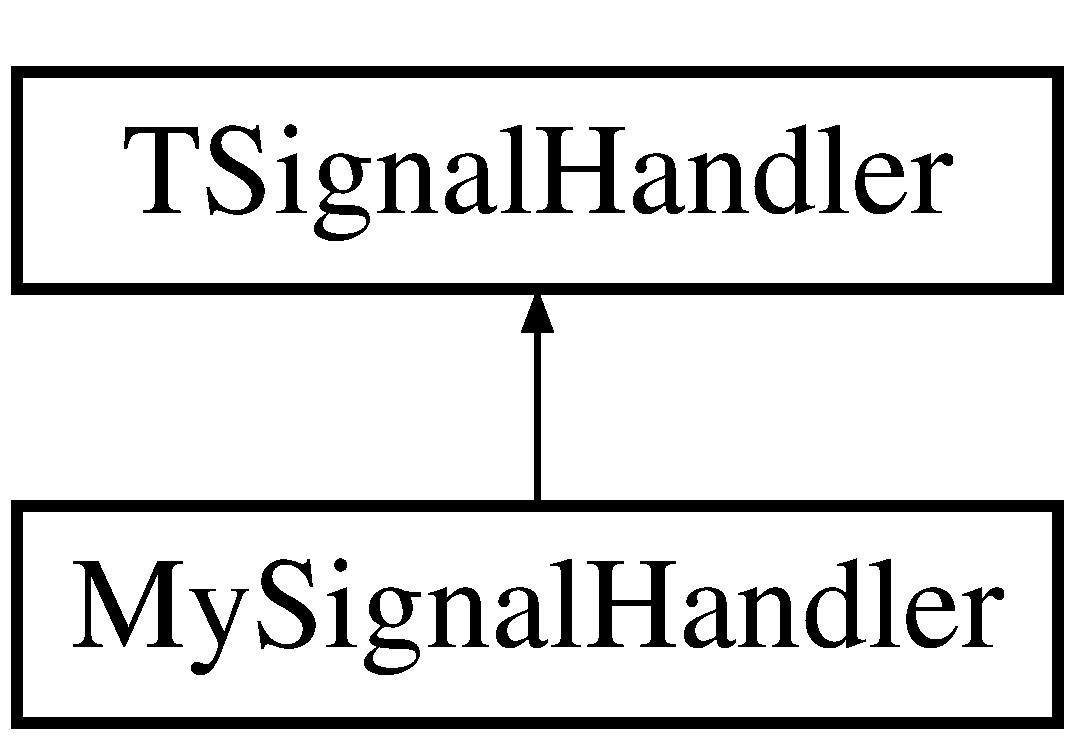
\includegraphics[height=2.000000cm]{classMySignalHandler}
\end{center}
\end{figure}
\subsection*{Public Member Functions}
\begin{DoxyCompactItemize}
\item 
\hypertarget{classMySignalHandler_a999b062d66e959846881d8adc47e8c97}{{\bfseries My\-Signal\-Handler} (E\-Signals sig)}\label{classMySignalHandler_a999b062d66e959846881d8adc47e8c97}

\item 
\hypertarget{classMySignalHandler_ac5fcaa3a73fd39f00b7c43eca04901ea}{Bool\-\_\-t {\bfseries Notify} ()}\label{classMySignalHandler_ac5fcaa3a73fd39f00b7c43eca04901ea}

\end{DoxyCompactItemize}


The documentation for this class was generated from the following files\-:\begin{DoxyCompactItemize}
\item 
include/My\-Signal\-Handler.\-h\item 
src/My\-Signal\-Handler.\-cc\end{DoxyCompactItemize}

\hypertarget{classUnpacker}{\section{Unpacker Class Reference}
\label{classUnpacker}\index{Unpacker@{Unpacker}}
}
\subsection*{Public Member Functions}
\begin{DoxyCompactItemize}
\item 
\hypertarget{classUnpacker_a53a5996d1d237b7472c6fa8f7cc154cf}{void {\bfseries Init\-Unpacker} (int opt, char $\ast$file\-\_\-name)}\label{classUnpacker_a53a5996d1d237b7472c6fa8f7cc154cf}

\item 
\hypertarget{classUnpacker_a3b6f311883854730c9457918643df096}{void {\bfseries Process} (\hyperlink{classDataSource}{Data\-Source} \&my\-\_\-src\-\_\-data)}\label{classUnpacker_a3b6f311883854730c9457918643df096}

\item 
\hypertarget{classUnpacker_a895addb324d545ad0777ecfd5631a1f5}{void {\bfseries Close} ()}\label{classUnpacker_a895addb324d545ad0777ecfd5631a1f5}

\item 
\hypertarget{classUnpacker_a7f332b859549c31037c8f81b9b4afb05}{void {\bfseries Load\-Parameters} (char $\ast$file\-\_\-name)}\label{classUnpacker_a7f332b859549c31037c8f81b9b4afb05}

\item 
\hypertarget{classUnpacker_aee0e1898faf8397ce110277c4d183c27}{void {\bfseries Fill\-Histograms} ()}\label{classUnpacker_aee0e1898faf8397ce110277c4d183c27}

\item 
\hypertarget{classUnpacker_ae49de8b0697861a0eda852bce8355b11}{bool {\bfseries Is\-Valid\-Fee64\-Id} ()}\label{classUnpacker_ae49de8b0697861a0eda852bce8355b11}

\item 
\hypertarget{classUnpacker_a1d30cfdd34ed107ffe4ddcd9f9efb533}{bool {\bfseries Is\-Valid\-Fee64\-Id} (int mod\-\_\-id)}\label{classUnpacker_a1d30cfdd34ed107ffe4ddcd9f9efb533}

\item 
\hypertarget{classUnpacker_a0f858d24727475892e49046e284b6fef}{void {\bfseries Update\-Histograms} ()}\label{classUnpacker_a0f858d24727475892e49046e284b6fef}

\item 
\hypertarget{classUnpacker_ac500c9f9ead3a36b053a38798addbc01}{void {\bfseries Write\-Histograms} ()}\label{classUnpacker_ac500c9f9ead3a36b053a38798addbc01}

\item 
\hypertarget{classUnpacker_abfbdbd6b4def8fc4030e9bd2c1f3f508}{void {\bfseries Reset\-Histograms} ()}\label{classUnpacker_abfbdbd6b4def8fc4030e9bd2c1f3f508}

\item 
\hypertarget{classUnpacker_ab981d52cb1876d8108d77ff455d7e358}{void {\bfseries Reset\-Data} ()}\label{classUnpacker_ab981d52cb1876d8108d77ff455d7e358}

\item 
\hypertarget{classUnpacker_a04de7adbe901e12f740b12cd2b1be623}{void {\bfseries Set\-B\-Debug} (bool flag)}\label{classUnpacker_a04de7adbe901e12f740b12cd2b1be623}

\item 
\hypertarget{classUnpacker_af05932a3e50a9234457acf25537fc5dc}{void {\bfseries Set\-B\-Histograms} (bool flag)}\label{classUnpacker_af05932a3e50a9234457acf25537fc5dc}

\item 
\hypertarget{classUnpacker_ab8a8cb19713467a6df11d79ed461dcb1}{void {\bfseries Set\-B\-Push\-Data} (bool flag)}\label{classUnpacker_ab8a8cb19713467a6df11d79ed461dcb1}

\item 
\hypertarget{classUnpacker_ac86398aca8a0b95fd4712f26349e672b}{void {\bfseries Set\-B\-Fill\-Tree} (bool flag)}\label{classUnpacker_ac86398aca8a0b95fd4712f26349e672b}

\item 
\hypertarget{classUnpacker_aca2a7ed3f8dc024d1066536afa8740a4}{void {\bfseries Set\-B\-Root\-Tree} (bool flag)}\label{classUnpacker_aca2a7ed3f8dc024d1066536afa8740a4}

\item 
\hypertarget{classUnpacker_af3edade6673717d03a1e57eaa1470a1e}{void {\bfseries Set\-B\-Sync\-Status} (bool flag)}\label{classUnpacker_af3edade6673717d03a1e57eaa1470a1e}

\item 
\hypertarget{classUnpacker_a29c14d8de773f4b2fea554834bf9eeac}{void {\bfseries Set\-Tm\-Stp} ()}\label{classUnpacker_a29c14d8de773f4b2fea554834bf9eeac}

\item 
\hypertarget{classUnpacker_a9dcb70fef617ebe64768edf57929dca8}{void {\bfseries Set\-Flags} ()}\label{classUnpacker_a9dcb70fef617ebe64768edf57929dca8}

\item 
\hypertarget{classUnpacker_ac86b7c6f573081f2d25933f59e99ad2a}{void {\bfseries Set\-Corr\-Scaler} (unsigned long value)}\label{classUnpacker_ac86b7c6f573081f2d25933f59e99ad2a}

\item 
\hypertarget{classUnpacker_a89bf86b9060b0c86179a09f16b1e42ac}{void {\bfseries Set\-Tm\-Stp\-Lsb} (unsigned long value)}\label{classUnpacker_a89bf86b9060b0c86179a09f16b1e42ac}

\item 
\hypertarget{classUnpacker_a14db23a0c6a42b90ceedf0d6eedcde56}{void {\bfseries Set\-Info\-Field} (unsigned long value)}\label{classUnpacker_a14db23a0c6a42b90ceedf0d6eedcde56}

\item 
\hypertarget{classUnpacker_a5654ec8872d662a8b8e08e028702904f}{void {\bfseries Set\-Adc\-Data} (unsigned int value)}\label{classUnpacker_a5654ec8872d662a8b8e08e028702904f}

\item 
\hypertarget{classUnpacker_a002ae77af3e8ef815227f84bd3c87dcc}{void {\bfseries Set\-Sample\-Length} (unsigned int value)}\label{classUnpacker_a002ae77af3e8ef815227f84bd3c87dcc}

\item 
\hypertarget{classUnpacker_a560ebee766ca8a64bedba7e63d6d0923}{void {\bfseries Set\-Data\-Type} (unsigned char value)}\label{classUnpacker_a560ebee766ca8a64bedba7e63d6d0923}

\item 
\hypertarget{classUnpacker_ac508e9c02bab43780627cc3c524cf170}{void {\bfseries Set\-Fee64\-Id} (unsigned char value)}\label{classUnpacker_ac508e9c02bab43780627cc3c524cf170}

\item 
\hypertarget{classUnpacker_a2b43b0eeb5e955119a74a46318255fae}{void {\bfseries Set\-Ch\-Id} (unsigned char value)}\label{classUnpacker_a2b43b0eeb5e955119a74a46318255fae}

\item 
\hypertarget{classUnpacker_abda952e6219fb87c334c06c50b0d3cd5}{void {\bfseries Set\-Adc\-Range} (unsigned char value)}\label{classUnpacker_abda952e6219fb87c334c06c50b0d3cd5}

\item 
\hypertarget{classUnpacker_a0117e3acc89039202fe59040fcd0dd0b}{void {\bfseries Set\-Info\-Code} (unsigned char value)}\label{classUnpacker_a0117e3acc89039202fe59040fcd0dd0b}

\item 
\hypertarget{classUnpacker_acf9e2327cce0a0de7b129022eaa6bcfa}{unsigned long {\bfseries Get\-Tm\-Stp} ()}\label{classUnpacker_acf9e2327cce0a0de7b129022eaa6bcfa}

\item 
\hypertarget{classUnpacker_a9266d8ad4fa81f8cda7a53b53b260563}{unsigned long {\bfseries Get\-Corr\-Scaler} ()}\label{classUnpacker_a9266d8ad4fa81f8cda7a53b53b260563}

\item 
\hypertarget{classUnpacker_a0bd57b059f49eb46126c4d54426b12e8}{unsigned long {\bfseries Get\-Tm\-Stp\-Lsb} ()}\label{classUnpacker_a0bd57b059f49eb46126c4d54426b12e8}

\item 
\hypertarget{classUnpacker_a5b1f803c59722d133e76b5ef87c35326}{unsigned long {\bfseries Get\-Info\-Field} ()}\label{classUnpacker_a5b1f803c59722d133e76b5ef87c35326}

\item 
\hypertarget{classUnpacker_a63dbc8a839bb58afde9b36a5ca3ffefc}{unsigned int {\bfseries Get\-Adc\-Data} ()}\label{classUnpacker_a63dbc8a839bb58afde9b36a5ca3ffefc}

\item 
\hypertarget{classUnpacker_a3662a0ce856d8ec304034df92b9f36c1}{unsigned int {\bfseries Get\-Sample\-Length} ()}\label{classUnpacker_a3662a0ce856d8ec304034df92b9f36c1}

\item 
\hypertarget{classUnpacker_ac9ec02e150d4115be7dfeee71567e12a}{unsigned char {\bfseries Get\-Data\-Type} ()}\label{classUnpacker_ac9ec02e150d4115be7dfeee71567e12a}

\item 
\hypertarget{classUnpacker_a8ee897d621a53befedc32d5384b0c227}{unsigned char {\bfseries Get\-Fee64\-Id} ()}\label{classUnpacker_a8ee897d621a53befedc32d5384b0c227}

\item 
\hypertarget{classUnpacker_ac084a3676f09ec7aa05c2b8e2710a5e7}{unsigned char {\bfseries Get\-Ch\-Id} ()}\label{classUnpacker_ac084a3676f09ec7aa05c2b8e2710a5e7}

\item 
\hypertarget{classUnpacker_a31e46b0efe0a16b3701f0860f0b53a09}{unsigned char {\bfseries Get\-Adc\-Range} ()}\label{classUnpacker_a31e46b0efe0a16b3701f0860f0b53a09}

\item 
\hypertarget{classUnpacker_a7ab50f7127241926a5eb675a96cba7d6}{unsigned char {\bfseries Get\-Info\-Code} ()}\label{classUnpacker_a7ab50f7127241926a5eb675a96cba7d6}

\item 
\hypertarget{classUnpacker_abca434c3e9a641db2a8a4a353875aa12}{bool {\bfseries Get\-Sync\-Flag} ()}\label{classUnpacker_abca434c3e9a641db2a8a4a353875aa12}

\item 
\hypertarget{classUnpacker_a0ed770f0343e73f88036fb3e5b372247}{bool {\bfseries Get\-B\-Sync\-Status} ()}\label{classUnpacker_a0ed770f0343e73f88036fb3e5b372247}

\item 
\hypertarget{classUnpacker_a5fe5ec240ec2a7965e03966457f94cb8}{bool {\bfseries Get\-B\-Push\-Data} ()}\label{classUnpacker_a5fe5ec240ec2a7965e03966457f94cb8}

\item 
\hypertarget{classUnpacker_a81ef25deecd85d687ad403a1ac23fd29}{bool {\bfseries Get\-B\-Fill\-Tree} ()}\label{classUnpacker_a81ef25deecd85d687ad403a1ac23fd29}

\item 
\hypertarget{classUnpacker_a7f640b2c85df12142ccc83789b182b2c}{bool {\bfseries Get\-B\-Histograms} ()}\label{classUnpacker_a7f640b2c85df12142ccc83789b182b2c}

\item 
\hypertarget{classUnpacker_a4aae1d6c81119c2fc21d3e241ad44f57}{bool {\bfseries Get\-B\-Debug} ()}\label{classUnpacker_a4aae1d6c81119c2fc21d3e241ad44f57}

\item 
\hypertarget{classUnpacker_af78cfcb511af3ae2eda1639f5c417601}{bool {\bfseries Get\-B\-Root\-Tree} ()}\label{classUnpacker_af78cfcb511af3ae2eda1639f5c417601}

\end{DoxyCompactItemize}
\subsection*{Public Attributes}
\begin{DoxyCompactItemize}
\item 
\hypertarget{classUnpacker_a753f76f4bfaed2983bb63e58a96f0c4d}{T\-Canvas $\ast$ {\bfseries c\-Unp1}}\label{classUnpacker_a753f76f4bfaed2983bb63e58a96f0c4d}

\item 
\hypertarget{classUnpacker_a05ebe860a3ed47535820b9ba46654cda}{T\-H1\-I $\ast$ {\bfseries h\-F\-E\-E64\-\_\-\-A\-D\-Clow}}\label{classUnpacker_a05ebe860a3ed47535820b9ba46654cda}

\item 
\hypertarget{classUnpacker_ac188f35b78b0ef1cb4220cbcc0577cf9}{T\-H1\-I $\ast$ {\bfseries h\-F\-E\-E64\-\_\-\-A\-D\-Chigh}}\label{classUnpacker_ac188f35b78b0ef1cb4220cbcc0577cf9}

\item 
\hypertarget{classUnpacker_ae99f11e8676eb6b1f89545a935e2522f}{T\-H1\-I $\ast$ {\bfseries h\-F\-E\-E64\-\_\-\-Waveform}}\label{classUnpacker_ae99f11e8676eb6b1f89545a935e2522f}

\item 
\hypertarget{classUnpacker_a80a1f5185a2bd496c2aad018fef11560}{T\-H1\-I $\ast$ {\bfseries h\-F\-E\-E64\-\_\-\-Info}}\label{classUnpacker_a80a1f5185a2bd496c2aad018fef11560}

\item 
\hypertarget{classUnpacker_a6257ddfe696ea7ab80422685ef3e6b12}{T\-H2\-I $\ast$ {\bfseries h\-Info\-Code\-\_\-\-F\-E\-E64}}\label{classUnpacker_a6257ddfe696ea7ab80422685ef3e6b12}

\item 
\hypertarget{classUnpacker_a4128fbf5d36f1fa371af66189cf87f7c}{T\-H1\-I $\ast$ {\bfseries h\-F\-E\-E64\-\_\-\-P\-A\-U\-S\-E}}\label{classUnpacker_a4128fbf5d36f1fa371af66189cf87f7c}

\item 
\hypertarget{classUnpacker_a39aa8f6dc232be2213453f7ddfc4d631}{T\-H1\-I $\ast$ {\bfseries h\-F\-E\-E64\-\_\-\-R\-E\-S\-U\-M\-E}}\label{classUnpacker_a39aa8f6dc232be2213453f7ddfc4d631}

\item 
\hypertarget{classUnpacker_a198d504be49a75ecbeadc1ed8a321cfa}{T\-H1\-I $\ast$ {\bfseries h\-F\-E\-E64\-\_\-\-S\-Y\-N\-C100}}\label{classUnpacker_a198d504be49a75ecbeadc1ed8a321cfa}

\item 
\hypertarget{classUnpacker_af67d4704ade07c9cf4ad17d6e90ce741}{T\-H2\-I $\ast$ {\bfseries h\-Ch\-\_\-\-F\-E\-E64\-\_\-\-A\-D\-Clow}}\label{classUnpacker_af67d4704ade07c9cf4ad17d6e90ce741}

\item 
\hypertarget{classUnpacker_ada79a2742e6a21f5c9cee46074ac2a5b}{T\-H2\-I $\ast$ {\bfseries h\-Ch\-\_\-\-F\-E\-E64\-\_\-\-A\-D\-Chigh}}\label{classUnpacker_ada79a2742e6a21f5c9cee46074ac2a5b}

\item 
\hypertarget{classUnpacker_a2a01879ac931f3dbf2ce4bbc5297eff4}{T\-H2\-I $\ast$ {\bfseries h\-Ch\-\_\-\-F\-E\-E64\-\_\-\-D\-I\-S\-C}}\label{classUnpacker_a2a01879ac931f3dbf2ce4bbc5297eff4}

\end{DoxyCompactItemize}


The documentation for this class was generated from the following files\-:\begin{DoxyCompactItemize}
\item 
include/Unpacker.\-h\item 
src/Unpacker.\-cpp\end{DoxyCompactItemize}

\chapter{File Documentation}
\hypertarget{Analysis_8h}{\section{include/\-Analysis.h File Reference}
\label{Analysis_8h}\index{include/\-Analysis.\-h@{include/\-Analysis.\-h}}
}
{\ttfamily \#include $<$iostream$>$}\\*
{\ttfamily \#include $<$T\-Tree.\-h$>$}\\*
{\ttfamily \#include $<$T\-Canvas.\-h$>$}\\*
{\ttfamily \#include $<$T\-H2.\-h$>$}\\*
{\ttfamily \#include $<$T\-H1.\-h$>$}\\*
{\ttfamily \#include \char`\"{}Calibrator.\-h\char`\"{}}\\*
{\ttfamily \#include \char`\"{}Data\-Source.\-h\char`\"{}}\\*
{\ttfamily \#include \char`\"{}Common.\-h\char`\"{}}\\*
\subsection*{Classes}
\begin{DoxyCompactItemize}
\item 
class \hyperlink{classAnalysis}{Analysis}
\begin{DoxyCompactList}\small\item\em A brief description of the class. \end{DoxyCompactList}\end{DoxyCompactItemize}

\hypertarget{Analysis_8cpp}{\section{src/\-Analysis.cpp File Reference}
\label{Analysis_8cpp}\index{src/\-Analysis.\-cpp@{src/\-Analysis.\-cpp}}
}
{\ttfamily \#include \char`\"{}Analysis.\-h\char`\"{}}\\*
{\ttfamily \#include $<$iomanip$>$}\\*
{\ttfamily \#include $<$stdio.\-h$>$}\\*
{\ttfamily \#include $<$string$>$}\\*

%--- End generated contents ---

% Index
\newpage
\phantomsection
\addcontentsline{toc}{part}{Index}
\printindex

\end{document}
